\chapter{METODOLOGÍA DE LA INVESTIGACIÓN}
\section{Diseño de la investigación}
En esta sección del documento se explica cuál fue el diseño, el tipo y el enfoque del trabajo de
investigación, así como también la población y la muestra. 

\subsection{Enfoque de la investigación}
El presente trabajo tuvo un enfoque cuantitativo ya que se busca diseñar y desarrollar instrumentos, en este caso modelos predictivos, para responder al problema estudiado a partir de medición de datos históricos en la plataforma Kickstarter con herramientas basadas en la estadística y matemáticas que puedan ser interpretadas por cualquier investigador. 

\subsection{Alcance de la investigación}
El alcance del presente trabajo fue descriptivo ya que se recolectaron datos en un determinado rango de tiempo (desde 2009 hasta el presente año 2019) para describir el comportamiento de las campañas de proyectos tecnológicos en Kickstarter a partir de las características de sus variables y con ello, pronosticar su posible éxito o fracaso antes de finalizar la campaña con un nivel óptimo de precisión.

\subsection{Tipo de la investigación}
Para determinar el tipo de la investigación, primero fue necesario definir el actual trabajo como Diseño Experimental ya que las variables que se tienen serán controladas, es decir, fueron agregadas o removidas en los modelos construidos en el experimento para analizar el impacto que estos tuvieron en los resultados obtenidos. Dentro de esta categoría se clasifica como Diseño Experimental Puro ya que se buscó medir la variable dependiente, en este caso \textit{state} (el estado actual del proyecto en Kickstarter) a partir de la manipulación de las demás variables independientes agregando o desagregándolas para comparar los rendimientos obtenidos de los instrumentos de medición y determinar cuáles de ellas finalmente fueron tomadas en cuenta.

\subsection{Descripción del prototipo de investigación}
Teniendo como referencia investigaciones basadas en Aprendizaje Profundo Multimodal, es decir, que combinan distintas características de una campaña de crowdfunding (\cite{pr_kamath2018suplearn}, décimo antecedente; \cite{pr_jin2019dayssuccess}, decimotercer antecedente; \cite{pr_cheng2019deeplearning}, decimocuarto antecedente) usando Metainformación (\cite{pr_chen2013kickpredict}, primer antecedente; \cite{pr_mitra2014phrases}, segundo antecedente; \cite{pr_zhou2015projectdesc}, tercer antecedente; \cite{pr_chen2015predcrowd}, cuarto antecedente; \cite{pr_beckwith2016predcrowd}, quinto antecedente; \cite{pr_li2016predcrowd}, sexto antecedente; \cite{pr_yuan2016textanalytics}, séptimo antecedente; \cite{pr_sawhney2016usingLT}, octavo antecedente; \cite{pr_kaur2017socmedcrowd}, noveno antecedente; \cite{pr_kamath2018suplearn}, décimo antecedente; \cite{pr_yu2018deeplearning}, undécimo antecedente; \cite{pr_jin2019dayssuccess}, decimotercer antecedente; \cite{pr_cheng2019deeplearning}, decimocuarto antecedente), descripción del proyecto (\cite{pr_mitra2014phrases}, segundo antecedente; \cite{pr_zhou2015projectdesc}, tercer antecedente; \cite{pr_yuan2016textanalytics}, séptimo antecedente; \cite{pr_sawhney2016usingLT}, octavo antecedente; \cite{pr_lee2018contentDL}, duodécimo antecedente; \cite{pr_jin2019dayssuccess}, decimotercer antecedente; \cite{pr_cheng2019deeplearning}, decimocuarto antecedente; \cite{pr_chen2019keywords_crowdfunding}, decimoquinto antecedente; \cite{pr_chaichi2019nlp_3dprinting}, decimosexto antecedente) y comentarios de los patrocinadores acerca del mismo (\cite{pr_chen2015predcrowd}, cuarto antecedente; \cite{pr_li2016predcrowd}, sexto antecedente; \cite{pr_lee2018contentDL}, duodécimo antecedente; \cite{pr_jin2019dayssuccess}, decimotercer antecedente; \cite{pr_shafqat2019topicpredictions}, decimoséptimo antecedente), la idea del prototipo final consistió en ensamblar estas 3 partes en un modelo apilado. Para ello, se representa cada una de las tres partes agrupadas en el marco de trabajo de la Figura \ref{3:fig1}.
\begin{figure}[htbp]
	\begin{center}
		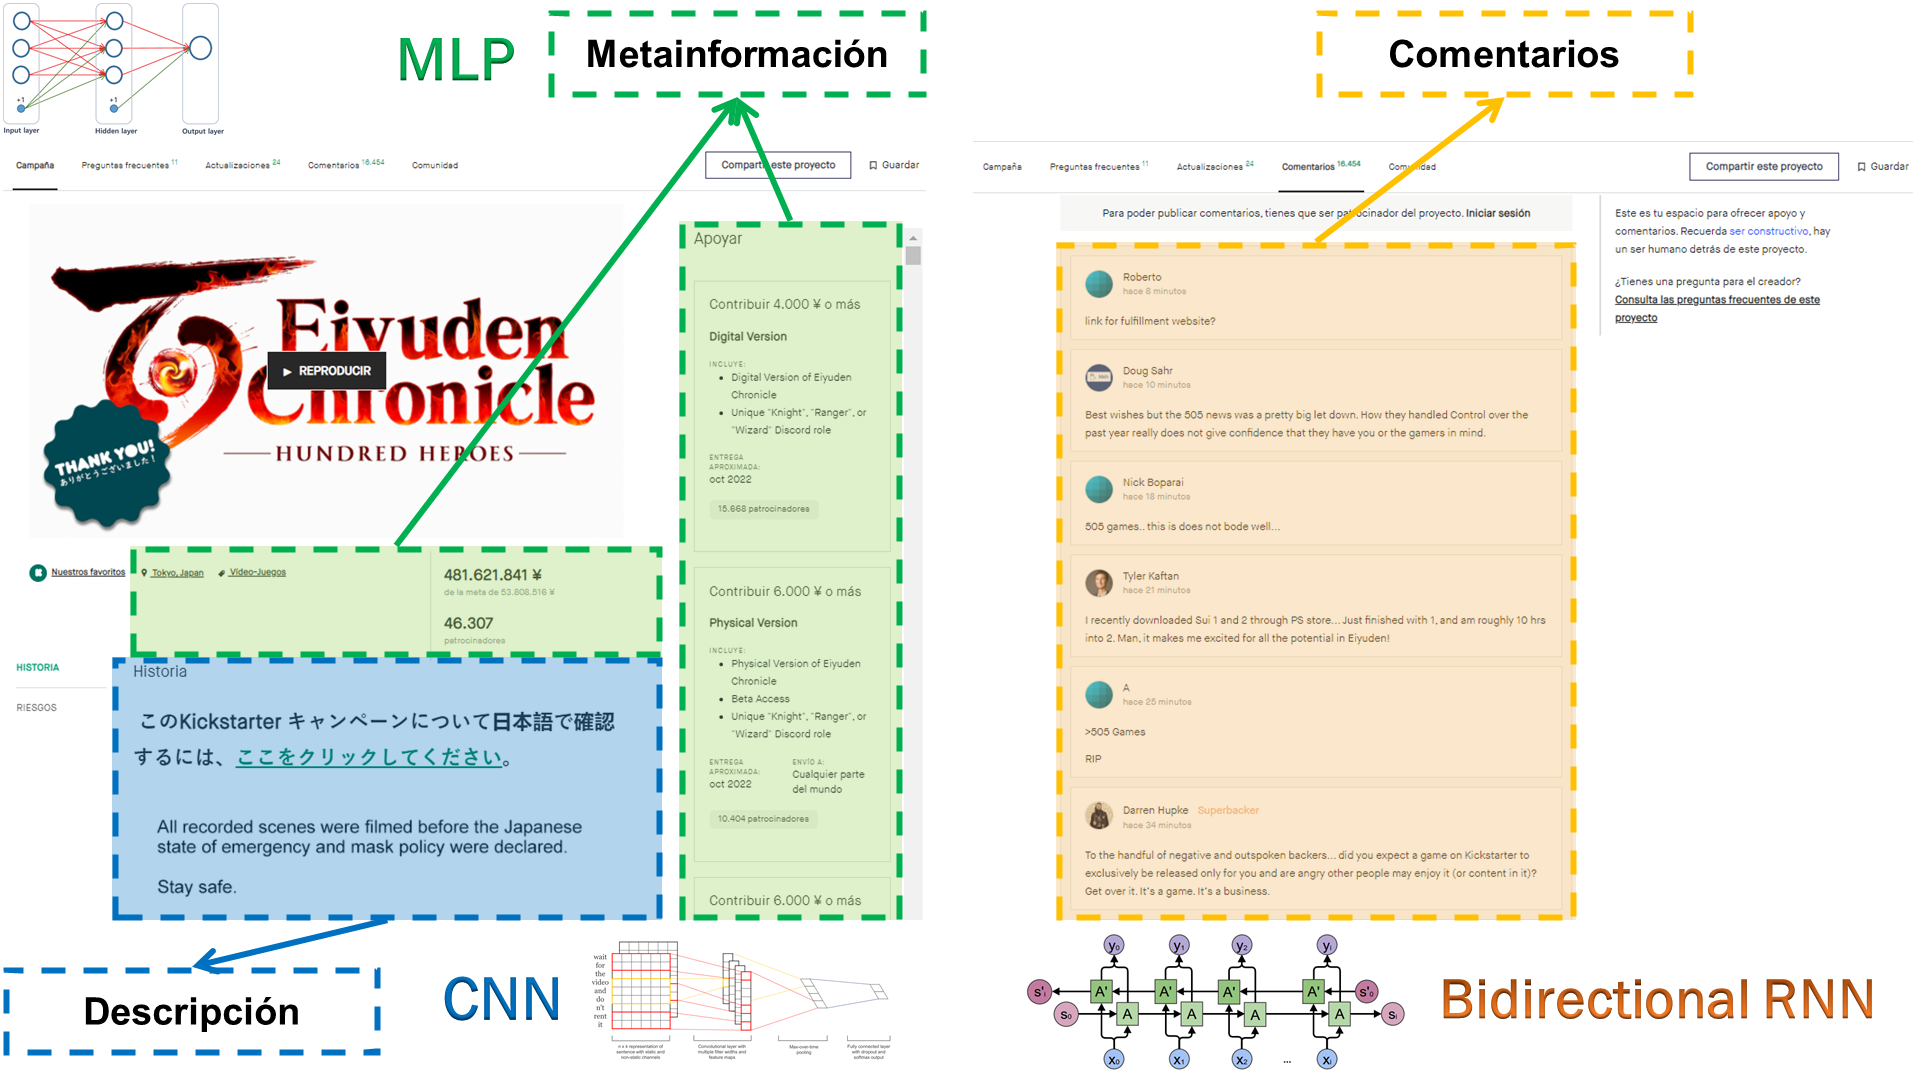
\includegraphics[width=1\textwidth]{3/figures/framework.png}
		\caption[Marco de trabajo del prototipo final]{Marco de trabajo del prototipo final.\\
		Fuente: Elaboración propia}
		\label{3:fig1}
	\end{center}
\end{figure}

\section{Población y muestra}

\subsection{Población}
La población fueron todos los proyectos de la web de crowdfunding Kickstarter.

\subsection{Muestra}
La muestra fueron 27,251 proyectos, incluyendo exitosos y fracasados, de la categoría Tecnología, de la web de crowdfunding Kickstarter, entre los periodos 2009 y 2019.

\subsection{Unidad de análisis}
La unidad de análisis fue un proyecto en Kickstarter de la categoría Tecnología entre los periodos 2009-2019.

\section{Operacionalización de Variables}
En la Tabla \ref{3:table1} se presentan las variables usadas para el conjunto de datos final basado en contenido textual y metainformación. Estas fueron seleccionadas de acuerdo al Benchmarking aplicado a los 17 antecedentes en el Capítulo II.

\begin{table}[h!]
	\caption[Diccionario de datos del conjunto final entrenado]{Diccionario de datos del conjunto final entrenado.}
	\label{3:table1}
	\centering
	\small
	\begin{tabular}{ |m{3cm}|m{10cm}|m{2cm}|  }
		\hline
		\rowcolor{bluejean}
		\Centering \color{white}{Variable}& \Centering \color{white}{Detalle}& \Centering \color{white}{Tipo de dato}\\
		\hline
		\rowcolor{turq}
		\multicolumn{3}{c}{Variables independientes} \\
		\hline
		\textbf{goal} &	Monto de la meta de financiamiento del proyecto. &	float64 \\
		\hline
		\textbf{completeness} & Porcentaje de financiamiento o completitud. & float64 \\
		\hline
		\textbf{duration} &	Duración de la campaña (en días). &	int64 \\
		\hline
		\textbf{pledges\_num} &	Cantidad de montos disponibles para contribuir. &	int64 \\
		\hline
		\textbf{pledged} &	Monto contribuído en la campaña. &	float64 \\
		\hline
		\textbf{pledges\_median} &	Mediana de montos disponibles para contribuir. &	float64 \\
		\hline
		\textbf{description} &	Descripción del proyecto. &	object \\
		\hline
		\textbf{comments} & Comentarios de patrocinadores sobre el proyecto. & object \\
		\hline
		\rowcolor{turq}
		\multicolumn{3}{c}{Variable dependiente} \\
		\hline
		\textbf{state} & Estado de financiamiento del proyecto. & object \\
		\hline
	\end{tabular}
	\par	%%Salto de linea
	\bigskip
	\begin{flushleft}	%%Alinear a la izquierda sin justificar
		\small Fuente: Elaboración propia.
	\end{flushleft}
\end{table}

Los autores citados por cada variable utilizada se mencionan a continuación:
\begin{itemize}
	\item \textbf{goal}: \cite{pr_chen2013kickpredict}, \cite{pr_mitra2014phrases}, \cite{pr_zhou2015projectdesc}, \cite{pr_chen2015predcrowd}, \cite{pr_li2016predcrowd}, \cite{pr_yuan2016textanalytics}, \cite{pr_sawhney2016usingLT}, \cite{pr_kaur2017socmedcrowd}, \cite{pr_kamath2018suplearn}, \cite{pr_yu2018deeplearning}, \cite{pr_jin2019dayssuccess}, \cite{pr_cheng2019deeplearning}.
	\item \textbf{completeness}: \cite{pr_chen2015predcrowd}.
	\item \textbf{duration}: \cite{pr_mitra2014phrases}, \cite{pr_zhou2015projectdesc}, \cite{pr_li2016predcrowd}, \cite{pr_sawhney2016usingLT}, \cite{pr_kaur2017socmedcrowd}, \cite{pr_kamath2018suplearn}, \cite{pr_yu2018deeplearning}, \cite{pr_jin2019dayssuccess}.
	\item \textbf{pledges\_num}: \cite{pr_chen2013kickpredict}, \cite{pr_mitra2014phrases}, \cite{pr_chen2015predcrowd}, \cite{pr_yuan2016textanalytics}, \cite{pr_jin2019dayssuccess}.
	\item \textbf{pledged}: \cite{pr_chen2013kickpredict}, \cite{pr_li2016predcrowd}, \cite{pr_kamath2018suplearn}.
	\item \textbf{pledges\_median}: \cite{pr_chen2015predcrowd}*, \cite{pr_jin2019dayssuccess}*.
	\item \textbf{description}: \cite{pr_mitra2014phrases}, \cite{pr_zhou2015projectdesc}, \cite{pr_yuan2016textanalytics}, \cite{pr_sawhney2016usingLT}, \cite{pr_kamath2018suplearn}, \cite{pr_lee2018contentDL}, \cite{pr_jin2019dayssuccess}, \cite{pr_cheng2019deeplearning}, \cite{pr_chen2019keywords_crowdfunding}, \cite{pr_chaichi2019nlp_3dprinting}.
	\item \textbf{comments}: \cite{pr_li2016predcrowd}, \cite{pr_kaur2017socmedcrowd}, \cite{pr_lee2018contentDL}, \cite{pr_jin2019dayssuccess}.
\end{itemize}

Si bien en los respectivos antecedentes marcados en (*) figuran el promedio de los montos disponibles para patrocinar, se usó la mediana en vez de la media ya que presentó mejor performance en los experimentos.

\section{Instrumentos de medida}
Los instrumentos de medida que sirvieron para determinar la performance del o los modelos construidos en el experimento serán algunas de las métricas de clasificación de Machine Learning descritas en los papers tomados como antecedentes en el Capítulo II del presente trabajo y seleccionadas mediante Benchmarking considerando como criterio la similitud del problema y propuestas de solución más aproximadas. Antes de proceder a explicar detalladamente cada una de ellas, es necesario conocer los conceptos de la Matriz de confusión, así como sus elementos que la componen.

\begin{itemize}
	\item \textbf{Matriz de confusión}: Es una tabla de NxN que resume el nivel de éxito de las predicciones de un modelo de clasificación; es decir, la correlación que existe entre la etiqueta y la clasificación del modelo. Un eje de una matriz de confusión es la etiqueta que el modelo predijo; el otro es la etiqueta real. N representa el número de clases. Es un problema de clasificación binaria, N=2 \parencite{gl_kohavi1998ml_glossary}. Su principal objetivo es describir el rendimiento de un modelo supervisado de Machine Learning en los datos de prueba, donde se desconocen los verdaderos valores. Se le llama “matriz de confusión” porque hace que sea fácil detectar dónde el sistema está confundiendo dos clases \parencite{gl_bigdata2019metricas}. Se representa de la siguiente manera:
	
	\begin{table}[h!]
		\caption[Matriz de confusión]{Matriz de confusión.}
		\label{3:table2}
		\centering
		\small
		\begin{tabular}{llcc}
			&                                                            & \multicolumn{2}{c}{\textbf{Valores Actuales}}                                                      \\ \cline{3-4} 
			& \multicolumn{1}{l|}{}                                      & \multicolumn{1}{c|}{\cellcolor[HTML]{DAEEF3}Positivos (1)} & \multicolumn{1}{c|}{\cellcolor[HTML]{DAEEF3}Negativos (0)} \\ \cline{2-4} 
			\multicolumn{1}{c|}{}                                             & \multicolumn{1}{c|}{\cellcolor[HTML]{DAEEF3}Positivos (1)} & \multicolumn{1}{c|}{Verdaderos Positivos (VP)}             & \multicolumn{1}{c|}{Falsos Positivos (FP)}                 \\ \cline{2-4} 
			\multicolumn{1}{c|}{\multirow{-2}{*}{\textbf{Valores Predichos}}} & \multicolumn{1}{c|}{\cellcolor[HTML]{DAEEF3}Negativos (0)} & \multicolumn{1}{c|}{Falsos Negativos (FN)}                 & \multicolumn{1}{c|}{Verdaderos Negativos (VN)}             \\ \cline{2-4} 
		\end{tabular}
		\par	%%Salto de linea
		\bigskip
		\begin{flushleft}	%%Alinear a la izquierda sin justificar
			\small Fuente: \cite{gl_izco2018bdc}
		\end{flushleft}
	\end{table}
	
\end{itemize}

De la Tabla \ref{3:table2}, existen 4 elementos clave:
\begin{itemize}
	\item \textbf{Verdadero positivo} (TP o \textit{True Positive}): Es el ejemplo en el que el modelo predijo de manera correcta la clase positiva. Por ejemplo, el modelo infirió correctamente que un paciente con determinadas características descritas en las variables sufre de cáncer \parencite{gl_google2018machinelearning}.
	\item \textbf{Verdadero negativo} (TN o \textit{True Negative}): Es el ejemplo en el que el modelo predijo de manera correcta la clase negativa. Por ejemplo, el modelo infirió correctamente que una determinada especie animal de acuerdo a sus características no era un mamífero \parencite{gl_google2018machinelearning}.
	\item \textbf{Falso positivo} (FP, \textit{False Positive} o Error del Tipo I): Es el ejemplo en el que el modelo predijo de manera incorrecta la clase positiva. Por ejemplo, el modelo infirió que un paciente varón presentaba embarazo (clase positiva) cuando en realidad no era así \parencite{gl_google2018machinelearning}.
	\item \textbf{Falso negativo} (FN, \textit{False Negative} o Error del Tipo II): Es el ejemplo en el que el modelo predijo de manera incorrecta la clase negativa. Por ejemplo, el modelo infirió que un mensaje de correo electrónico en particular no era spam (clase negativa), pero ese mensaje en realidad sí era spam \parencite{gl_google2018machinelearning}. 
\end{itemize}

Explicado los conceptos anteriores, se derivan las siguientes métricas de clasificación usadas comúnmente, de las cuales serán usadas solo las 3 primeras tomando como referencia los papers de los antecentes:
\begin{itemize}
	\item \textbf{Exactitud} (\textit{accuracy}): Representa la fracción de predicciones que se realizaron correctamente sobre el total de ejemplos en un modelo de clasificación. Se determina mediante la siguiente fórmula \parencite{gl_kohavi1998ml_glossary}:
	
	%\begin{equcaption}[!ht]
	\begin{equation}\label{eq:accuracy}
	\phantomsection
	Exactitud=\frac{V.P.+V.N.}{V.P.+V.N.+F.P.+F.N.}
	\end{equation}
	\myequations{Fórmula para calcular la exactitud}
	%\caption[Fórmula para calcular la exactitud]{Fórmula para calcular la exactitud. Fuente: \cite{gl_kohavi1998ml_glossary}}
	%\end{equcaption}
	
	Esta métrica responde a la pregunta ¿Cuál es la proporción de predicciones que se realizaron correctamente? \parencite{gl_izco2018bdc}
	
	\item \textbf{Precisión} (\textit{precision}): Representa el número de elementos identificados correctamente como positivo de un total de elementos identificados como positivos \parencite{gl_bigdata2019metricas}. Se calcula mediante la siguiente fórmula:
	
	%\begin{equcaption}[!ht]
	\begin{equation}\label{eq:precision}
	\phantomsection
	Precisi\acute{o}n=\frac{V.P.}{V.P.+F.P.}
	\end{equation}
	\myequations{Fórmula para calcular la precisión}
	%\caption[Fórmula para calcular la precisión]{Fórmula para calcular la precisión. Fuente: \cite{gl_kohavi1998ml_glossary}}
	%\end{equcaption}
	
	Esta métrica responde a la pregunta ¿Qué proporción de predicciones positivas es correcta? \parencite{gl_izco2018bdc}
	
	\item \textbf{Área bajo la curva ROC} (\textit{AUC}): Considera todos los umbrales de clasificación posibles. Representa la probabilidad de que un clasificador tenga más seguridad de que un ejemplo resulte ser un verdadero positivo con respecto a que sea un falso positivo \parencite{gl_google2018machinelearning}. Para entender el concepto del área, se necesita entender qué es la curva ROC y para qué sirve en primer lugar.
	
	La curva ROC permite cuantificar la performance de distinción entre dos cosas del modelo como, por ejemplo, si un paciente tiene cáncer o no.
	
	Siguiendo el anterior ejemplo, se tiene un modelo que predice si un paciente sufre de cáncer o no, cuyo resultado es el siguiente (Figura \ref{3:fig2})
	
	\begin{figure}[htbp]
		\begin{center}
			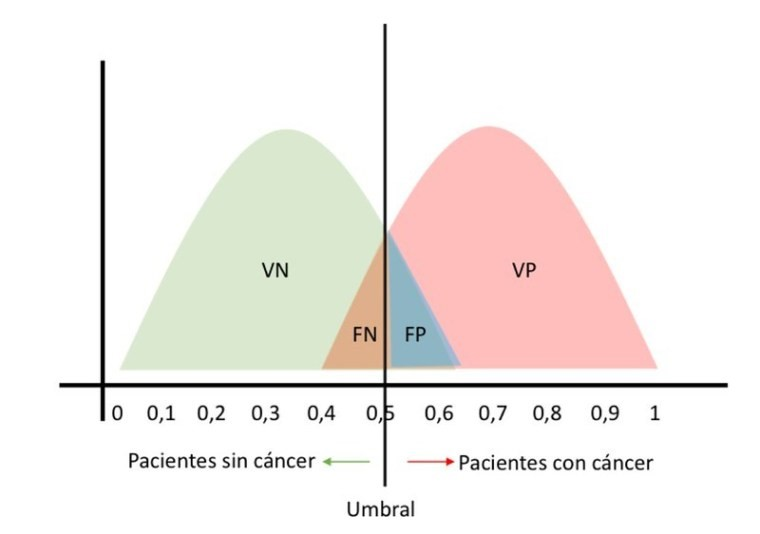
\includegraphics[width=0.50\textwidth]{3/figures/auc_example.jpg}
			\caption[Descripción de resultados de modelo descriptivo de ejemplo]{Descripción de resultados de modelo descriptivo de ejemplo.\\
			Fuente: \cite{gl_gonzalez2019auc}}
			\label{3:fig2}
		\end{center}
	\end{figure}
	
	En esta imagen, se puede observar que el área de borde verde (que contiene a los Falsos Positivos y el total de Negativos) representa a todos los pacientes que no tienen cáncer, mientras que el área de borde rojo (que contiene a los Falsos Negativos y el total de Positivos) representa a todos los pacientes que sí tienen cáncer. El umbral, que está establecido con valor 0.5, representa el punto de corte en el que el modelo clasificará a todos los pacientes por encima de ese valor como positivos, es decir, que sí tienen cáncer; mientras que aquellos por debajo del valor del umbral serán clasificados como negativos, es decir, que no tienen cáncer.
	
	Cuando el umbral se desplaza hacia la izquierda, es decir, cuando la sensibilidad aumenta, la especificidad disminuirá. Por el contrario, cuando el umbral se desplaza hacia la derecha, la sensibilidad disminuirá y la especificidad aumentará. Se concluye entonces que existe una relación inversa entre la sensibilidad y la especificidad. En la curva ROC se representa la sensitividad (1-especificidad) \parencite{gl_gonzalez2019auc}.
	
	Ahora bien, el área que se grafica bajo esta curva explicará qué tan bien funciona el modelo. Este tendrá un mejor desempeño si la curva se aleja de la diagonal principal como se observa en la Figura \ref{3:fig3}.
	
	\begin{figure}[htbp]
		\begin{center}
			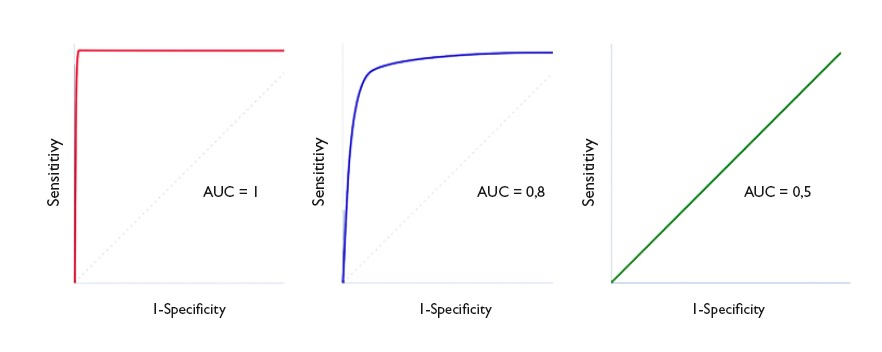
\includegraphics[width=0.75\textwidth]{3/figures/auc_curves.jpg}
			\caption[Comparación de tres resultados de la curva AUC en el modelo]{Comparación de tres resultados de la curva AUC en el modelo.\\
			Fuente: \cite{gl_molina2017pediatria_curvaroc}}
			\label{3:fig3}
		\end{center}
	\end{figure}
	
	Una interpretación básica del área bajo la curva ROC respecto del poder discriminante del modelo se muestra a continuación \parencite{bk_britos2006datamining}:
	\begin{itemize}
		\item Si el área bajo la curva ROC = 0.5, entonces el poder discriminante del modelo es nulo.
		\item Si el área bajo la curva 0.5 $<$ ROC $<$ 0.7, entonces el poder discriminante del modelo no es aceptable.
		\item Si el área bajo la curva 0.7 $\leq$ ROC $<$ 0.8, entonces el poder discriminante del modelo es aceptable.
		\item Si el área bajo la curva 0.8 $\leq$ ROC $<$ 0.9, entonces el poder discriminante del modelo es excelente.
		\item Si el área bajo la curva ROC $\geq$ 0.9, entonces el poder discriminante del modelo es excepcionalmente bueno.
	\end{itemize}
	\item \textbf{Sensibilidad} (\textit{recall}, \textit{sensitivity} o \textit{True Positive Rate}): Representa el número de elementos correctamente identificados como positivos del total de positivos verdaderos \parencite{gl_bigdata2019metricas}. Se calcula mediante la siguiente fórmula:
	
	%\begin{equcaption}[!ht]
	\begin{equation}\label{eq:recall}
	\phantomsection
	Sensibilidad=\frac{V.P.}{V.P.+F.N.}
	\end{equation}
	\myequations{Fórmula para calcular la sensibilidad}
	%\caption[Fórmula para calcular la sensibilidad]{Fórmula para calcular la sensibilidad. Fuente: \cite{gl_kohavi1998ml_glossary}}
	%\end{equcaption}
	
	\item \textbf{Puntaje F1} (\textit{F1-Score}): Representa la media armónica de la precisión y la sensibilidad. Normalmente, se usa cuando uno difiere mucho del otro y no es posible realizar una conclusión determinante ya que solo es posible predecir bien una clase \parencite{gl_bigdata2019metricas}. Se calcula mediante la siguiente fórmula:
	
	%\begin{equcaption}[!ht]
	\begin{equation}\label{eq:f1-score}
	\phantomsection
	Puntaje F1=\frac{2*Precisi\acute{o}n*Sensibilidad}{Precisi\acute{o}n+Sensibilidad}
	\end{equation}
	\myequations{Fórmula para calcular el puntaje F1}
	%\caption[Fórmula para calcular el puntaje F1]{Fórmula para calcular el puntaje F1. Fuente: \cite{gl_kohavi1998ml_glossary}}
	%\end{equcaption}
	
\end{itemize}

\clearpage

\section{Técnicas de recolección de datos}
Los conjuntos de datos recolectados para la investigación se componen de mezcla de observaciones cuantitativas (variables numéricas basadas en características del proyecto como la meta de financiamiento, montos prometidos, duración de la campaña y otros indicadores financieros) y cualitativas (descripción y comentarios del proyecto). Para obtener los 3 principales datasets, se siguió el flujo de la Figura \ref{3:fig4}. La base de datos de la metainformación, que comprende las variables cuantitativas y propaganda del proyecto, fue consolidada luego de descargar un histórico público de 10 años de la página web “Web Robots”, fundada por los ex corporativos de TI Tomás Vitulskis y Paulius Jonaitis, y posteriormente pre-procesarla. Mientras que por el lado de la descripción y comentarios de cada proyecto, se usaron técnicas y herramientas de \textit{web scraping} a partir de los URLs. El detalle de cada paso del proceso se explica en la sección de Construcción de los conjuntos finales de datos del Capítulo IV.

\begin{figure}[h]
	\begin{center}
		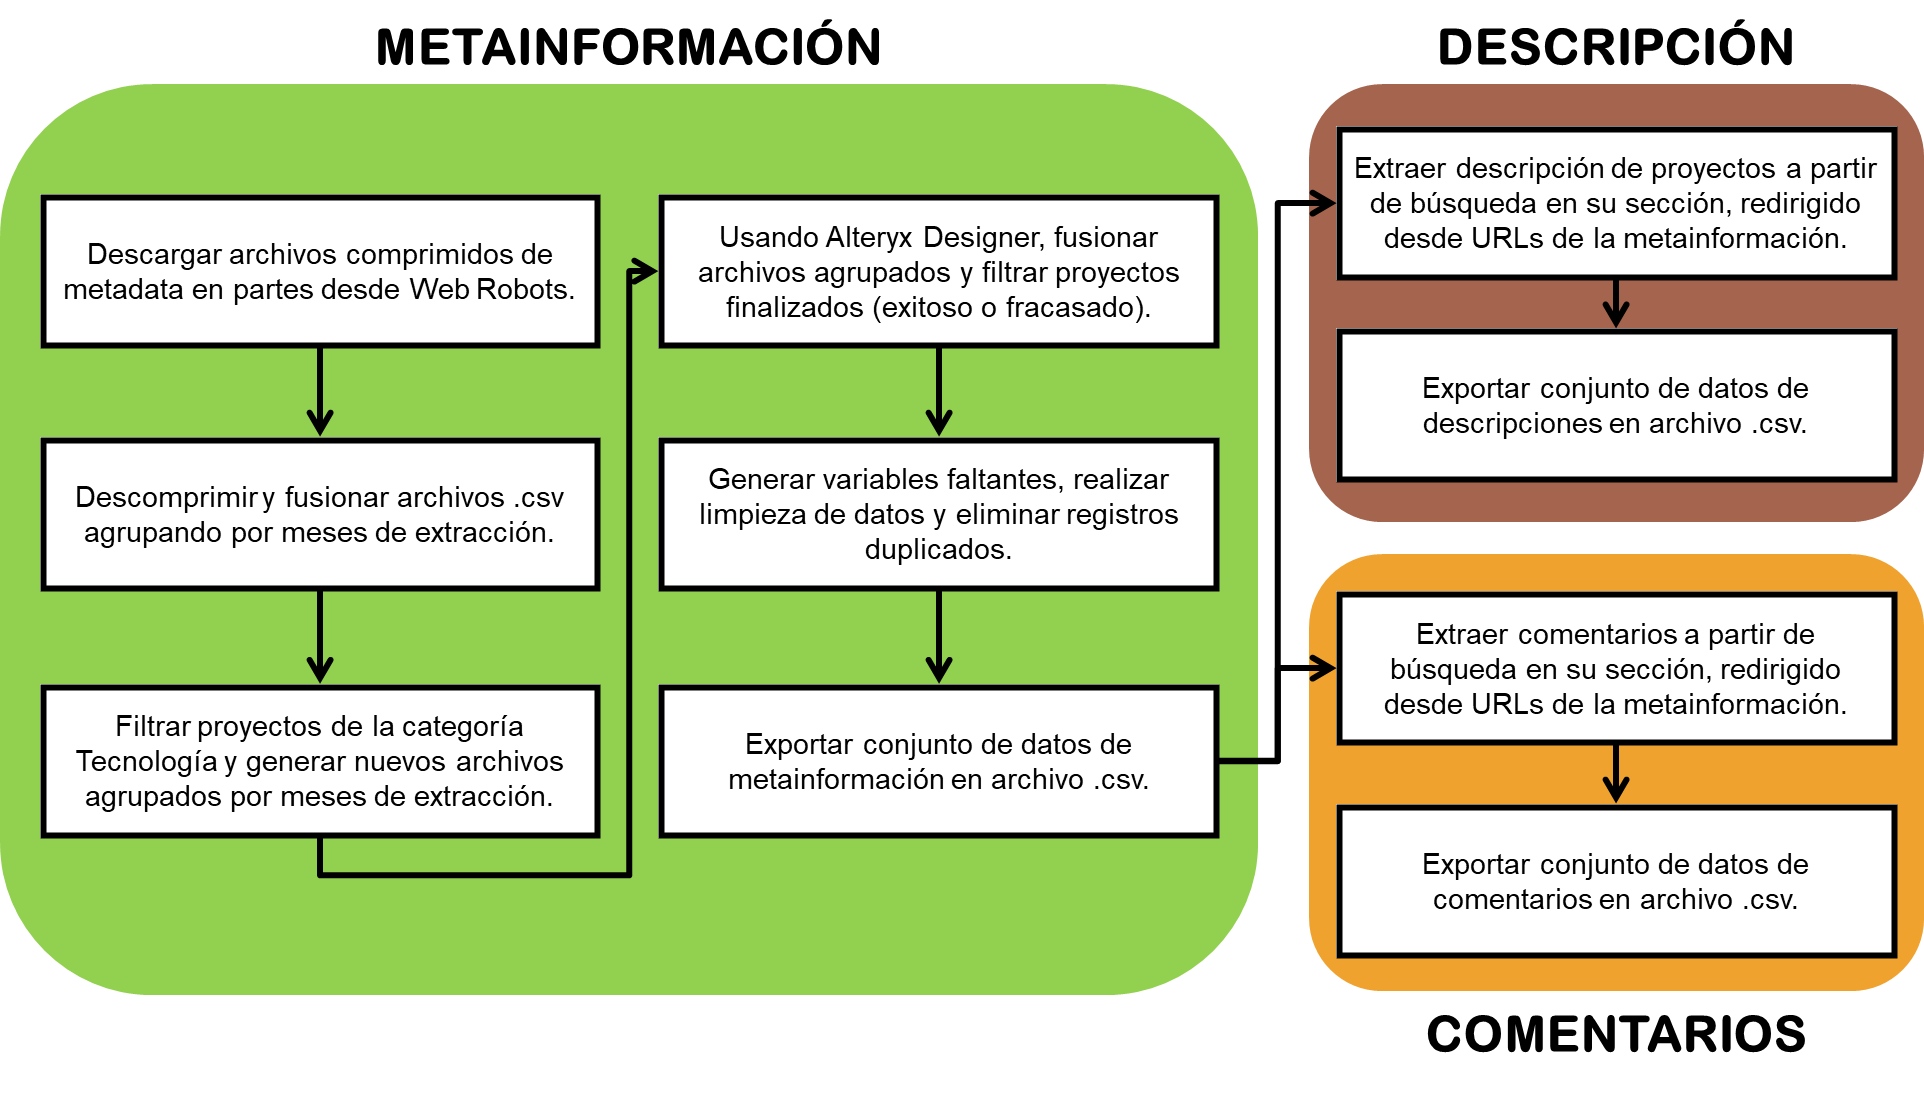
\includegraphics[width=0.95\textwidth]{3/figures/data_recolection_flux.png}
		\caption[Flujograma de la recolección de conjuntos finales de datos]{Flujograma de la recolección de conjuntos finales de datos.\\
		Fuente: Elaboración propia.}
		\label{3:fig4}
	\end{center}
\end{figure}

Asimismo, para encontrar algunos de los papers con la información requerida más cercana, se utilizaron keywords o palabras clave como \textit{crowdfunding}, \textit{Machine Learning}, \textit{Deep Learning}, \textit{prediction}, \textit{Kickstarter}, \textit{accuracy} y \textit{projects}.

\section{Técnicas para el procesamiento y análisis de la información}
Como se explicó en el punto 2.2.6 del Marco Teórico del presente trabajo, dentro de los sistemas de analítica de negocio, Big Data y Minería de Datos, tres de las metodologías más usadas son CRISP-DM, SEMMA y KDD \parencite{tec_braulio2015metodologiasdm}.

Después de evaluar y comparar las tres mencionadas, se concluyó que la mejor de ellas dependerá de la intención o finalidad que busca lograr el o los involucrados en el negocio tanto en objetivos como en resultados. Para la presente investigación, se siguió la metodología de CRISP-DM debido a la coyuntura en la que se desarrolló. Las razones de la elección de la misma fueron las siguientes:

\begin{itemize}
	\item La metodología CRISP-DM contempla entre sus fases la comprensión del negocio además de la parte técnica que incluye el modelado y análisis de resultados. La comprensión del negocio tiene un rol importante ya que se define al inicio de todo el proceso para dar el alcance del proyecto y definir objetivos que se buscan a partir de la Minería de Datos y Big Data.
	\item Ayuda a la gerencia del proyecto en la planeación y toma de decisiones (fase Despliegue) a partir de los resultados obtenidos, reportándolos y convirtiéndolos en oportunidades a considerar en los objetivos del negocio.
	\item Evalúa en todo el proceso los datos y variables usadas con el fin de crear el mejor modelo. Las variables seleccionadas serán importantes para interpretar los resultados y tomar decisiones.
	\item Si se habla de las otras dos metodologías, empezando por KDD, si bien esta contempla 9 pasos durante su proceso, el objetivo de KDD en cada uno de estos resulta ser más técnico, es decir, trabajar, seleccionar e interpretar métricas, variables, modelos, entre otros para obtener los mejores resultados más allá de considerar el contexto y comprensión del negocio. De hecho, no existe alguna fase dedicada al entendimiento del mismo.
	\item Por otra parte, la metodología SEMMA se basa, como su nombre lo indica, en la selección, exploración y modelado de grandes cantidades de datos para descubrir patrones de negocio desconocidos. Sin embargo, al limitarse a 5 fases comenzando con la fase de muestreo, no hace hincapié en la comprensión del negocio, sino más bien comienza con el procesamiento de datos para la construcción del modelo.
\end{itemize}

Cada una de las fases de la metodología seleccionada se detalla a continuación.

\subsection{Comprensión del negocio}
La primera fase de la metodología CRISP-DM consiste en la definición del problema de Minería de Datos que se tiene, así como el entendimiento de los objetivos y requerimientos que se espera lograr en el proyecto.

Para empezar, el crowdfunding se basa, como su nombre en inglés lo indica, en lograr que un proyecto emprendedor sea llevado a cabo gracias al financiamiento colectivo. Existen 4 diferentes modelos de crowdfunding: basado en donaciones, basado en recompensas, basado en capital social y basado en deuda. El crowdfunding basado en capital social se encuentra actualmente limitado en los Estados Unidos debido a que la Regulación D de la Ley de Valores de 1933 prohíbe la participación de muchos potenciales inversionistas y los obliga a tener un ingreso anual mayor a \$200,000 o más de \$1 millón en patrimonio neto \parencite{cr_lichtig2015crowdfunding}.

El modelo basado en donaciones se refiere a la recaudación de fondos a través de la Web 2.0, en el cual los patrocinadores no esperan recompensas materiales a cambio sino más bien una recompensa social. Por el contrario, el modelo basado en recompensas ofrece compensación tanto material como inmaterial y representa hoy en día el modelo de crowdfunding más frecuente. Los financiadores, por un lado, pueden verse beneficiados de la venta anticipada, recibiendo el proyecto o producto financiado antes de su publicación o entrada al mercado al mejor precio. Los proyectos que pertenecen a esta categoría a menudo son organizaciones sin fines de lucro \parencite{cr_kraus2016crowdfunding_strategies}.

Kickstarter, la plataforma de crowdfunding más citada, analizada y una de las más grandes, es una comunidad basada en el crowdfunding por recompensas. A la fecha, 128 mil proyectos han sido financiados, 3 billones de dólares fueron prometidos en proyectos y 13 millones de patrocinadores han participado, del cual el 31\% ha colocado dinero en más de 1 proyecto.

La particularidad de los proyectos en esta plataforma es que, luego de cumplir un plazo de tiempo determinado, el monto prometido acumulado puede ser asignado a los proyectos que hayan alcanzado o superado la meta estipulada al inicio. Para ello, los dueños de los proyectos tienen que crear estrategias para lograr campañas exitosas y hacer realidad su producto. Un 75\% de los proyectos que fueron apoyados por al menos 25 patrocinadores han sido financiados exitosamente \parencite{cr_kickstarter_learn}.

Para lograr que un proyecto en la plataforma logre impactar en la comunidad, debe contar con conexiones duraderas, retroalimentación del producto y ser tangible. Asimismo, algunos enfoques importantes se basan en probar nuevas ideas, aumentar la comunidad y cubrir costos de manufacturación.

Para empezar a realizar la campaña del proyecto, es necesario seguir las sugerencias basadas en los autores \cite{cr_yu2017kickstarter_course} y \cite{cr_kickstarter_intro}:
\begin{itemize}
	\item Identificar la meta óptima del proyecto. Se debe realizar una lista de todos los costos, así como el shipping que deben de cada país. También se debe contar con un buffer en caso ocurra un imprevisto. Se puede determinar la meta a través de la fórmula (Gastos + Buffer) x Alcance.
	\item Crear el video de la campaña en un presupuesto. El vídeo resulta ser un factor muy importante ya que aquellos que cuentan con un video de su proyecto tienen un 50\% de chance de tener éxito. El promedio debería ser de 3.38 minutos, aunque el público presta más atención hacia aquellos que duran poco. El vídeo debe contener y responder las siguientes preguntas:
	\begin{itemize}
		\item ¿Qué hace memorable al proyecto?
		\item ¿Cómo se verá el proyecto?
		\item ¿Por qué se está creando el producto?
		\item ¿Por qué lo necesitas?
		\item ¿Por qué es importante que tu proyecto exista?
		\item ¿Por qué debes ser tú su creador?
		\item ¿Por qué tu compañía?
		\item ¿Cómo proveerás una solución?
		\item ¿Cómo funciona la solución?
	\end{itemize}
	Es importante destacar las estadísticas del problema que se piensa resolver al inicio del video ya que el primer minuto resulta ser el lapso de tiempo que más capta la atención del público. Se recomienda también tener buen audio e iluminación.
	\item Escribir la descripción del proyecto. Otro factor clave en el desempeño de la campaña de un proyecto en Kickstarter resulta ser la descripción que representa un resumen de los puntos más relevantes del producto. Se debe mencionar una breve introducción del proyecto, cómo funciona, para quiénes son, el proceso que se siguió en el desarrollo, detalles y especificaciones, y un cronograma e hitos.
	\item Incluir imágenes sobre cómo lucirá el proyecto. Esta prueba convencerá a más de una persona en querer invertir en el proyecto. Las imágenes a veces atraen más a las personas que no gustan leer la descripción completa del proyecto.
	\item Determinar las recompensas del proyecto. Al basarse en un modelo de crowdfunding en recompensas, los patrocinadores esperan un beneficio por parte del proyecto una vez este logre alcanzar su financiamiento. El número ideal de recompensas puede ser entre 5 y 7. Una recompensa en promedio de \$100 es la que genera más dinero. Las recompensas pueden ser de cuatro tipos: el producto en sí mismo entregado hacia los patrocinadores antes que este salga al mercado, reconocimientos en la página web y acceso hacia actualizaciones, recuerdos y certificados de membresía, y nuevas experiencias como visita a los desarrolladores en sus estudios.
\end{itemize}

Todos los factores anteriormente mencionados determinarán en gran medida el nivel de éxito que tendrá un proyecto una vez su campaña sea lanzada en la plataforma.

\subsection{Comprensión de los datos}
Una vez comprendido el funcionamiento del negocio y sus objetivos que busca lograr, la siguiente fase fue entender el significado de los datos con los que se trabajaron. Estos incluyen valores y variables que determinaron la performance del modelo elaborado en las siguientes etapas.

Para ello, se analizaron estadísticamente las variables numéricas del dataset generado de la Metainformación (Tabla \ref{4:table1}) luego del proceso de construcción bajo el flujo de la Figura \ref{3:fig4} y que se explica en el subcapítulo 1 del Capítulo IV.

En el siguiente subcapítulo del mismo capítulo, se detalla el análisis exploratorio de cada variable, entre los cuales destaca el desbalance en las etiquetas de la variable dependiente a predecir (\textit{state}).

\subsection{Preparación de los datos}
El análisis exploratorio de los datos fue determinante para la selección final de variables de la Metainformación, gracias al uso de herramientas estadísticas como el análisis de correlaciones para discriminar aquellas que superaron el límite fijado y que desembocó, luego del pre-procesamiento detallado en el subcapítulo 3 del mismo capítulo, en la Tabla \ref{3:table1}.

\subsection{Modelamiento}
Luego del pre-procesamiento de los datos, en esta fase se procedió a crear modelos predictivos para cada modalidad considerada. Tomando de referencia a los antecedentes del Marco Teórico, los más usados para cada modalidad se detalla a continuación:
\begin{itemize}
	\item \textbf{Metainformación}: Perceptrón Multicapa (\cite{pr_kamath2018suplearn}, \cite{pr_yu2018deeplearning}, \cite{pr_cheng2019deeplearning}), Máquina de Vectores de Soporte (\cite{pr_chen2013kickpredict}, \cite{pr_beckwith2016predcrowd}, \cite{pr_sawhney2016usingLT}), Regresión Logística (\cite{pr_mitra2014phrases}, \cite{pr_zhou2015projectdesc}, \cite{pr_beckwith2016predcrowd}, \cite{pr_li2016predcrowd}, \cite{pr_kaur2017socmedcrowd}), Regresión Log-logística (\cite{pr_li2016predcrowd}), Bosques Aleatorios (\cite{pr_chen2015predcrowd}, \cite{pr_yuan2016textanalytics}, \cite{pr_kamath2018suplearn}), Árboles de Decisión (\cite{pr_beckwith2016predcrowd}, \cite{pr_kamath2018suplearn}), Naïve Bayes (\cite{pr_beckwith2016predcrowd}, \cite{pr_kamath2018suplearn}), Modelo Seq2seq (\cite{pr_jin2019dayssuccess}).
	\item \textbf{Descripción}: CNN (\cite{pr_cheng2019deeplearning}), LSTM (\cite{pr_jin2019dayssuccess}), Modelo Seq2seq (\cite{pr_lee2018contentDL}), Máquina de Vectores de Soporte o variantes (\cite{pr_sawhney2016usingLT}, \cite{pr_chen2019keywords_crowdfunding}), Regresión Logística (\cite{pr_mitra2014phrases}, \cite{pr_zhou2015projectdesc}), LDA o variantes (\cite{pr_yuan2016textanalytics}, \cite{pr_sawhney2016usingLT}).
	\item \textbf{Comentarios}: LSTM (\cite{pr_jin2019dayssuccess}, \cite{pr_shafqat2019topicpredictions}), LDA o variantes (\cite{pr_shafqat2019topicpredictions}), Modelo Seq2seq (\cite{pr_lee2018contentDL}, \cite{pr_jin2019dayssuccess}), HAN (\citeauthor{pr_lee2018contentDL}), Regresión Logística (\cite{pr_li2016predcrowd}, \cite{pr_kaur2017socmedcrowd}), Regresión Log-logística (\cite{pr_li2016predcrowd}).
\end{itemize}

De todos los modelos mencionados, los más predominantes de Aprendizaje Automático fueron las Máquinas de Vectores de Soporte y los de Regresión Logística, mientras que por el lado de Aprendizaje Profundo, fueron los Perceptrones Multicapa aunque las otras redes enunciadas derivan de este tipo.

Según los anteriores autores, salvo en investigaciones donde se usaron 1 sola modalidad, como por ejemplo la Metainformación, los modelos de Aprendizaje Profundo tuvieron mejor desempeño que los tradicionales de Aprendizaje Automático. Además, dado que la propuesta de esta investigación es ensamblar múltiples modelos, considerar un mix de ambos tipos de arquitectura resulta inviable por la complejidad de transformación de sus salidas de distintos tamaños.

Por ello, se optó por usar arquitecturas de Redes Neuronales para cada modalidad con el fin de poder ensamblar y comparar sus resultados, tanto de manera individual como en el modelo apilado, con la literatura.

\subsection{Evaluación}
De las métricas de clasificación de Aprendizaje Automático explicadas en el cuarto subcapítulo del presente capítulo, las usadas por los autores de la literatura fueron las siguientes:

\begin{itemize}
	\item \textbf{Exactitud}: \cite{pr_chen2013kickpredict} (primer antecedente); \cite{pr_chen2015predcrowd} (cuarto antecedente); \cite{pr_beckwith2016predcrowd} (quinto antecedente); \cite{pr_yuan2016textanalytics} (séptimo antecedente); \cite{pr_sawhney2016usingLT} (octavo antecedente); \cite{pr_kaur2017socmedcrowd} (noveno antecedente); \cite{pr_kamath2018suplearn} (décimo antecedente); \cite{pr_yu2018deeplearning} (undécimo antecedente); \cite{pr_lee2018contentDL} (duodécimo antecedente); \cite{pr_cheng2019deeplearning} (decimocuarto antecedente); \cite{pr_chen2019keywords_crowdfunding} (decimoquinto antecedente); \cite{pr_shafqat2019topicpredictions} (decimoséptimo antecedente).
	\item \textbf{Precisión}: \cite{pr_beckwith2016predcrowd} (quinto antecedente); \cite{pr_yuan2016textanalytics} (séptimo antecedente); \cite{pr_kaur2017socmedcrowd} (noveno antecedente); \cite{pr_cheng2019deeplearning} (decimocuarto antecedente).
	\item \textbf{Sensibilidad}: \cite{pr_beckwith2016predcrowd} (quinto antecedente); \cite{pr_yuan2016textanalytics} (séptimo antecedente); \cite{pr_kaur2017socmedcrowd} (noveno antecedente); \cite{pr_cheng2019deeplearning} (decimocuarto antecedente); \cite{pr_chen2019keywords_crowdfunding} (decimoquinto antecedente).
	\item \textbf{Especificidad}: \cite{pr_chen2019keywords_crowdfunding} (decimoquinto antecedente).
	\item \textbf{Ratio de Falsa Alarma}: \cite{pr_kaur2017socmedcrowd} (noveno antecedente).
	\item \textbf{Media Geométrica (G-Mean)}: \cite{pr_chen2019keywords_crowdfunding} (decimoquinto antecedente).
	\item \textbf{Puntaje F1}: \cite{pr_zhou2015projectdesc} (tercer antecedente); \cite{pr_beckwith2016predcrowd} (quinto antecedente); \cite{pr_yuan2016textanalytics} (séptimo antecedente); \cite{pr_kaur2017socmedcrowd} (noveno antecedente); \cite{pr_cheng2019deeplearning} (decimocuarto antecedente); \cite{pr_chen2019keywords_crowdfunding} (decimoquinto antecedente).
	\item \textbf{Curva ROC}: \cite{pr_zhou2015projectdesc} (tercer antecedente); \cite{pr_beckwith2016predcrowd} (quinto antecedente).
	\item \textbf{Área bajo la Curva ROC (AUC)}: \cite{pr_beckwith2016predcrowd} (quinto antecedente); \cite{pr_li2016predcrowd} (sexto antecedente); \cite{pr_kaur2017socmedcrowd} (noveno antecedente); \cite{pr_yu2018deeplearning} (undécimo antecedente); \cite{pr_cheng2019deeplearning} (decimocuarto antecedente).
	\item \textbf{Área bajo la Curva Precisión-Sensibilidad (PRC)}: \cite{pr_kaur2017socmedcrowd} (noveno antecedente).
	\item \textbf{Error de Validación Cruzada}: \cite{pr_mitra2014phrases} (segundo antecedente).
	\item \textbf{Coeficiente de Correlación de Matthew (MCC)}: \cite{pr_kaur2017socmedcrowd} (noveno antecedente).
	\item \textbf{Divergencia de Kullback-Leibler (KL)}: \cite{pr_jin2019dayssuccess} (decimotercer antecedente).
	\item \textbf{Raíz del Error Cuadrático Medio (RMSE)}: \cite{pr_jin2019dayssuccess} (decimotercer antecedente).
	\item \textbf{Error Absoluto Medio (MAE)}: \cite{pr_jin2019dayssuccess} (decimotercer antecedente).
	\item \textbf{Índice de Concordancia (CI)}: \cite{pr_jin2019dayssuccess} (decimotercer antecedente).
\end{itemize}

En el Capítulo 5 se explica cuáles fueron seleccionadas para evaluar cada modelo.

\subsection{Despliegue}
Luego de analizar el desempeño de cada modelo, tanto individual como el modelo final, se compararon los resultados con los antecedentes y se desarrolló una prueba piloto en la cual el modelo apilado entrenado fue ejecutado usando como entrada la URL de un proyecto aleatorio de Kickstarter para, luego de obtener sus características, predecir su estado de financiamiento. Esta acción también se encuentra detallada en el Capítulo 5.

\section{Cronograma de actividades y presupuesto}
Se elaboró un cronograma de actividades de toda la investigación, mostrada en la Figura \ref{3:fig5}, contemplando desde el inicio de la misma, desarrollo, evaluación de resultados y sustentación.
\begin{figure}[h]
	\begin{center}
		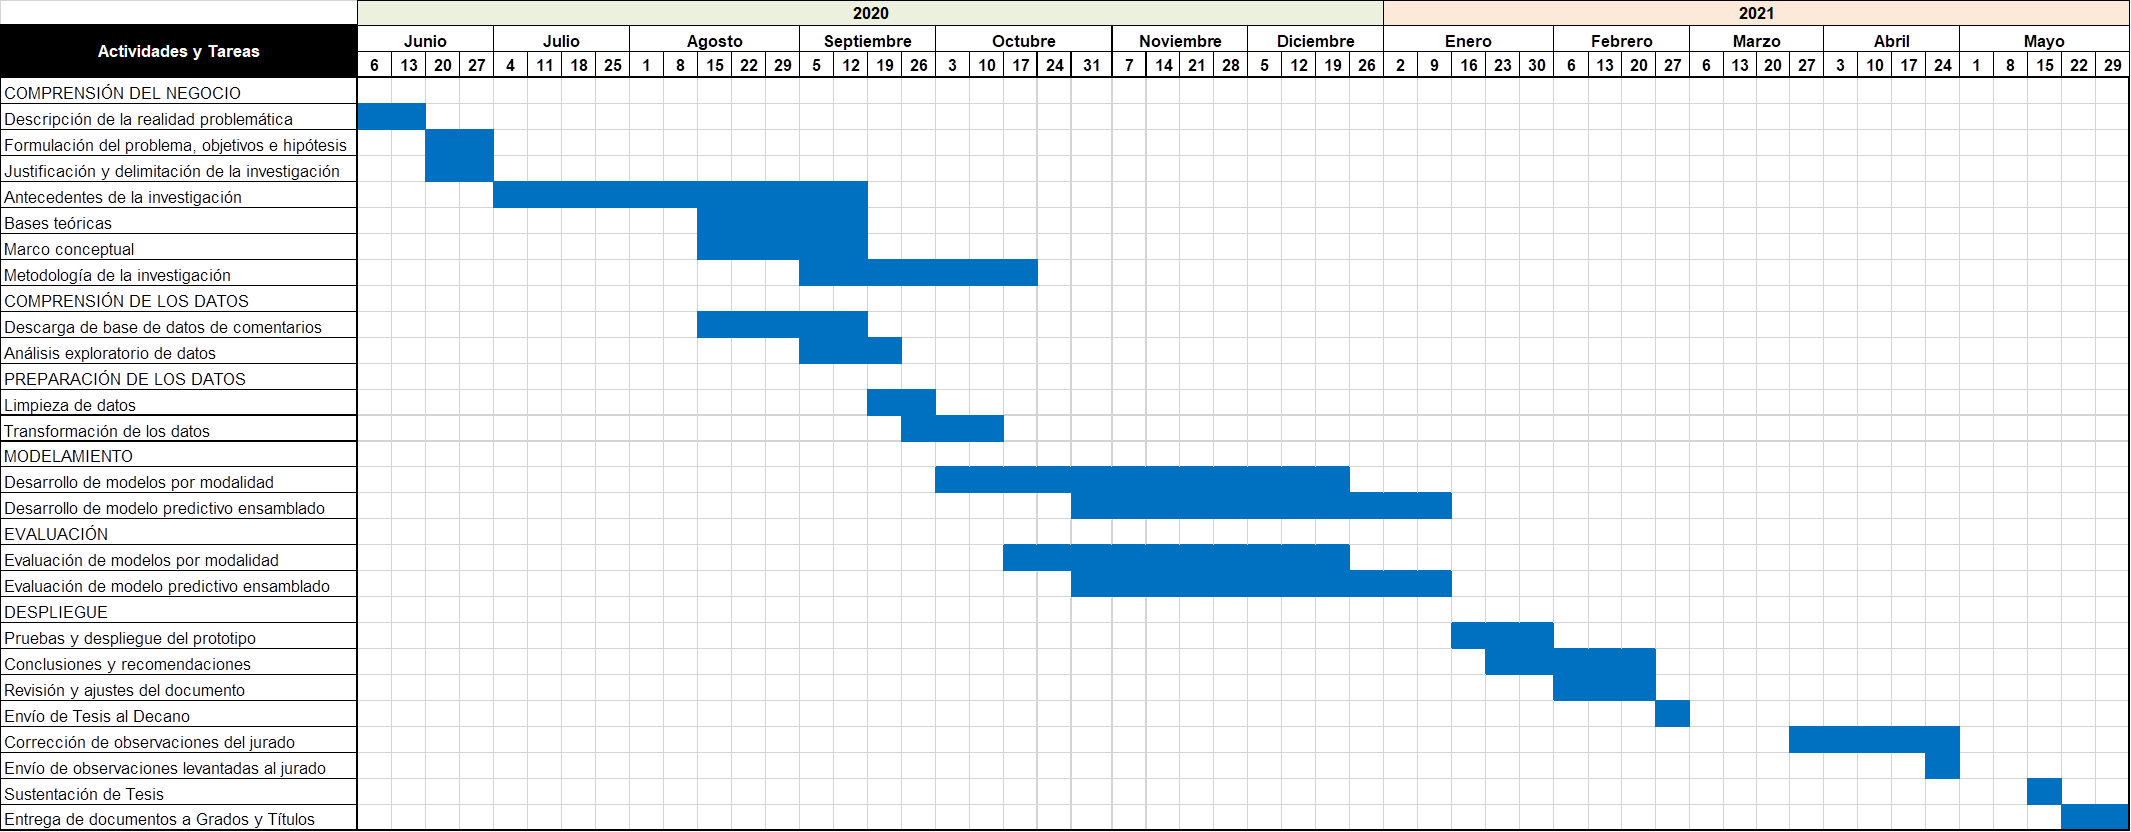
\includegraphics[width=1.1\textwidth]{3/figures/cronograma.png}
		\caption[Cronograma de actividades de la investigación]{Cronograma de actividades de la investigación.\\
		Fuente: Elaboración propia}
		\label{3:fig5}
	\end{center}
\end{figure}

La partida presupuestal de todo el proyecto se divide en dos partes: los costos personales del autor y los costos de las herramientas para la operación del proyecto.

Los costos personales del autor del trabajo de tesis se muestran en la Tabla \ref{3:table3}. Estos incluyen las herramientas adquiridas antes del inicio de la investigación como la laptop, así como los pagos de servicios generales y del trámite de elaboración y sustentación pública de Tesis. Se menciona la cantidad de horas utilizadas por el autor para el desarrollo del trabajo; sin embargo no se considera un valor monetario por cada unidad al ser un valor incalculable.

\begin{table}[h!]
	\caption[Presupuesto de los costos personales del autor]{Presupuesto de los costos personales del autor.}
	\label{3:table3}
	\centering
	\small
	\begin{tabular}{llrr}
		\rowcolor[HTML]{010066} 
		\multicolumn{1}{c}{\cellcolor[HTML]{010066}{\color[HTML]{FFFFFF} \textbf{Item}}} & \multicolumn{1}{c}{\cellcolor[HTML]{010066}{\color[HTML]{FFFFFF} \textbf{Tiempo usado (horas)}}} & \multicolumn{1}{c}{\cellcolor[HTML]{010066}{\color[HTML]{FFFFFF} \textbf{Costo (soles)}}} & \multicolumn{1}{c}{\cellcolor[HTML]{010066}{\color[HTML]{FFFFFF} \textbf{Subtotal}}}     \\
		\rowcolor[HTML]{DAE8FC} 
		\multicolumn{4}{l}{\cellcolor[HTML]{DAE8FC}\textbf{Recursos materiales}}                                                  \\
		Laptop Lenovo ideapad 330 Core i7 8va Gen  &  & S/.4,500.00 & S/.4,500.00 \\
		\rowcolor[HTML]{DAE8FC} 
		\multicolumn{4}{l}{\cellcolor[HTML]{DAE8FC}\textbf{Pagos del trámite de elaboración y sustentación pública de Tesis}}                                                                                                                                                                                                                                                \\
		Derecho de inscripción de tema de investigación &  & S/.800.00 & S/.800.00 \\
		Reserva del tema de tesis  &  & S/.2,700.00 & S/.2,700.00 \\
		Derecho de sustentación                                                          & & S/.1,500.00                                                                               & S/.1,500.00                                                                              \\
		\rowcolor[HTML]{DAE8FC} 
		\multicolumn{4}{l}{\cellcolor[HTML]{DAE8FC}\textbf{Recursos humanos}} \\
		Avance de tesis                                                                  & \multicolumn{1}{r}{900}                                                                    & Incalculable                                                                              & -                                                                                        \\
		\rowcolor[HTML]{DAE8FC} 
		\multicolumn{4}{l}{\cellcolor[HTML]{DAE8FC}\textbf{Servicios generales}}                                                   \\
		Internet + luz (7 meses)                                                         & \multicolumn{1}{r}{110}                                                                    & S/.80.00                                                                                  & S/.560.00                                                                              \\
		\rowcolor[HTML]{303498} 
		{\color[HTML]{FFFFFF} \textbf{Total}} & {\color[HTML]{FFFFFF} } & \multicolumn{1}{l}{\cellcolor[HTML]{303498}{\color[HTML]{FFFFFF} }} & \multicolumn{1}{l}{\cellcolor[HTML]{303498}{\color[HTML]{FFFFFF} \textbf{S/.10,060.00}}}
	\end{tabular}
	\par	%%Salto de linea
	\bigskip
	\begin{flushleft}	%%Alinear a la izquierda sin justificar
		\small Fuente: Fuente: Elaboración propia.
	\end{flushleft}
\end{table}

Asimismo, también se contemplan los costos por uso de servicios en la nube como parte de la extracción de comentarios desde servidores en Google Cloud Platform (GCP) y desarrollo de modelos en Google Colab Pro en la Tabla \ref{3:table4}.

\begin{table}[h!]
	\caption[Presupuesto de los costos de las herramientas para el proyecto]{Presupuesto de los costos de las herramientas para el proyecto.}
	\label{3:table4}
	\centering
	\small
	\begin{tabular}{llrrr}
		\rowcolor[HTML]{010066} 
		\multicolumn{1}{c}{\cellcolor[HTML]{010066}{\color[HTML]{FFFFFF} \textbf{Item}}} & \multicolumn{1}{c}{\cellcolor[HTML]{010066}{\color[HTML]{FFFFFF} \textbf{Unidades}}} & \multicolumn{1}{c}{\cellcolor[HTML]{010066}{\color[HTML]{FFFFFF} \textbf{Costo (dólares)}}} & \multicolumn{1}{l}{\cellcolor[HTML]{010066}{\color[HTML]{FFFFFF} \textbf{Horas}}} & \multicolumn{1}{c}{\cellcolor[HTML]{010066}{\color[HTML]{FFFFFF} \textbf{Subtotal}}} \\
		\rowcolor[HTML]{DAE8FC} 
		\multicolumn{4}{l}{\cellcolor[HTML]{DAE8FC}\textbf{Google Cloud Platform}}                                                                                                                                                                                                                                                                                & \textbf{-\$98.56}                                                                    \\
		Instancia VM Ubuntu (g1-small, 12GB RAM) & 1 & \$0.021 & 310 & \$6.51 \\
		Imagen de instancia Ubuntu & 8 & \$0.02 & 306 & \$48.96                                                                              \\
		Instancia VM de Windows Server 2019 (4GB RAM) & 1 & \$0.086 & 300 & \$25.80                                                                              \\
		Costo por instancias encendidas & 10 & & & \$3.41                                                                               \\
		Uso de instancias posteriormente eliminadas & & & & \$95.88                                                                              \\
		Pago mensual (luego de aceptar mejora de plan) & 4 & \$5.22 & & \$20.88                                                                              \\
		Crédito de \$300.00 por 12 meses & 1 & -\$300.00 & & -\$300.00                                                                            \\
		\rowcolor[HTML]{DAE8FC} 
		\multicolumn{4}{l}{\cellcolor[HTML]{DAE8FC}\textbf{Google Colab Pro}}                                                                                                                                                                                                                                                                                     & \textbf{\$49.95}                                                                     \\
		Pago mensual (luego de aceptar mejora de plan) & 5 & \$9.99 & \multicolumn{1}{l}{} & \$49.95                                                                              \\
		\rowcolor[HTML]{303498} 
		{\color[HTML]{FFFFFF} \textbf{Total a pagar}} & {\color[HTML]{FFFFFF}} & \multicolumn{1}{l}{\cellcolor[HTML]{303498}{\color[HTML]{FFFFFF} }} & \multicolumn{1}{l}{\cellcolor[HTML]{303498}} & {\color[HTML]{FFFFFF} \textbf{\$49.95}}                                             
	\end{tabular}
	\par	%%Salto de linea
	\bigskip
	\begin{flushleft}	%%Alinear a la izquierda sin justificar
		\small Fuente: Fuente: Elaboración propia.
	\end{flushleft}
\end{table}

Los montos totales por el uso de instancias creadas en GCP son descontados de los \$300.00 en crédito gratuito válidos por 12 meses (a la fecha en que se desarrolló la investigación) \parencite{ot_googlecloud_freetrial}, recibidos inicialmente desde el 12 de agosto del 2020 (fecha de inscripción) para poder ser usados como versión de prueba. A partir del siguiente mes, se mejoró el plan para habilitar más servicios (por ejemplo, máquina virtual en Windows) y comenzó a facturarse \$5.22 mensualmente.